% Options for packages loaded elsewhere
\PassOptionsToPackage{unicode}{hyperref}
\PassOptionsToPackage{hyphens}{url}
\PassOptionsToPackage{dvipsnames,svgnames,x11names}{xcolor}
%
\documentclass[
  12pt,
  letterpaper,
]{book}

\usepackage{amsmath,amssymb}
\usepackage{iftex}
\ifPDFTeX
  \usepackage[T1]{fontenc}
  \usepackage[utf8]{inputenc}
  \usepackage{textcomp} % provide euro and other symbols
\else % if luatex or xetex
  \usepackage{unicode-math}
  \defaultfontfeatures{Scale=MatchLowercase}
  \defaultfontfeatures[\rmfamily]{Ligatures=TeX,Scale=1}
\fi
\usepackage{lmodern}
\ifPDFTeX\else  
    % xetex/luatex font selection
\fi
% Use upquote if available, for straight quotes in verbatim environments
\IfFileExists{upquote.sty}{\usepackage{upquote}}{}
\IfFileExists{microtype.sty}{% use microtype if available
  \usepackage[]{microtype}
  \UseMicrotypeSet[protrusion]{basicmath} % disable protrusion for tt fonts
}{}
\makeatletter
\@ifundefined{KOMAClassName}{% if non-KOMA class
  \IfFileExists{parskip.sty}{%
    \usepackage{parskip}
  }{% else
    \setlength{\parindent}{0pt}
    \setlength{\parskip}{6pt plus 2pt minus 1pt}}
}{% if KOMA class
  \KOMAoptions{parskip=half}}
\makeatother
\usepackage{xcolor}
\usepackage[margin=1in]{geometry}
\setlength{\emergencystretch}{3em} % prevent overfull lines
\setcounter{secnumdepth}{5}
% Make \paragraph and \subparagraph free-standing
\makeatletter
\ifx\paragraph\undefined\else
  \let\oldparagraph\paragraph
  \renewcommand{\paragraph}{
    \@ifstar
      \xxxParagraphStar
      \xxxParagraphNoStar
  }
  \newcommand{\xxxParagraphStar}[1]{\oldparagraph*{#1}\mbox{}}
  \newcommand{\xxxParagraphNoStar}[1]{\oldparagraph{#1}\mbox{}}
\fi
\ifx\subparagraph\undefined\else
  \let\oldsubparagraph\subparagraph
  \renewcommand{\subparagraph}{
    \@ifstar
      \xxxSubParagraphStar
      \xxxSubParagraphNoStar
  }
  \newcommand{\xxxSubParagraphStar}[1]{\oldsubparagraph*{#1}\mbox{}}
  \newcommand{\xxxSubParagraphNoStar}[1]{\oldsubparagraph{#1}\mbox{}}
\fi
\makeatother

\usepackage{color}
\usepackage{fancyvrb}
\newcommand{\VerbBar}{|}
\newcommand{\VERB}{\Verb[commandchars=\\\{\}]}
\DefineVerbatimEnvironment{Highlighting}{Verbatim}{commandchars=\\\{\}}
% Add ',fontsize=\small' for more characters per line
\usepackage{framed}
\definecolor{shadecolor}{RGB}{241,243,245}
\newenvironment{Shaded}{\begin{snugshade}}{\end{snugshade}}
\newcommand{\AlertTok}[1]{\textcolor[rgb]{0.68,0.00,0.00}{#1}}
\newcommand{\AnnotationTok}[1]{\textcolor[rgb]{0.37,0.37,0.37}{#1}}
\newcommand{\AttributeTok}[1]{\textcolor[rgb]{0.40,0.45,0.13}{#1}}
\newcommand{\BaseNTok}[1]{\textcolor[rgb]{0.68,0.00,0.00}{#1}}
\newcommand{\BuiltInTok}[1]{\textcolor[rgb]{0.00,0.23,0.31}{#1}}
\newcommand{\CharTok}[1]{\textcolor[rgb]{0.13,0.47,0.30}{#1}}
\newcommand{\CommentTok}[1]{\textcolor[rgb]{0.37,0.37,0.37}{#1}}
\newcommand{\CommentVarTok}[1]{\textcolor[rgb]{0.37,0.37,0.37}{\textit{#1}}}
\newcommand{\ConstantTok}[1]{\textcolor[rgb]{0.56,0.35,0.01}{#1}}
\newcommand{\ControlFlowTok}[1]{\textcolor[rgb]{0.00,0.23,0.31}{\textbf{#1}}}
\newcommand{\DataTypeTok}[1]{\textcolor[rgb]{0.68,0.00,0.00}{#1}}
\newcommand{\DecValTok}[1]{\textcolor[rgb]{0.68,0.00,0.00}{#1}}
\newcommand{\DocumentationTok}[1]{\textcolor[rgb]{0.37,0.37,0.37}{\textit{#1}}}
\newcommand{\ErrorTok}[1]{\textcolor[rgb]{0.68,0.00,0.00}{#1}}
\newcommand{\ExtensionTok}[1]{\textcolor[rgb]{0.00,0.23,0.31}{#1}}
\newcommand{\FloatTok}[1]{\textcolor[rgb]{0.68,0.00,0.00}{#1}}
\newcommand{\FunctionTok}[1]{\textcolor[rgb]{0.28,0.35,0.67}{#1}}
\newcommand{\ImportTok}[1]{\textcolor[rgb]{0.00,0.46,0.62}{#1}}
\newcommand{\InformationTok}[1]{\textcolor[rgb]{0.37,0.37,0.37}{#1}}
\newcommand{\KeywordTok}[1]{\textcolor[rgb]{0.00,0.23,0.31}{\textbf{#1}}}
\newcommand{\NormalTok}[1]{\textcolor[rgb]{0.00,0.23,0.31}{#1}}
\newcommand{\OperatorTok}[1]{\textcolor[rgb]{0.37,0.37,0.37}{#1}}
\newcommand{\OtherTok}[1]{\textcolor[rgb]{0.00,0.23,0.31}{#1}}
\newcommand{\PreprocessorTok}[1]{\textcolor[rgb]{0.68,0.00,0.00}{#1}}
\newcommand{\RegionMarkerTok}[1]{\textcolor[rgb]{0.00,0.23,0.31}{#1}}
\newcommand{\SpecialCharTok}[1]{\textcolor[rgb]{0.37,0.37,0.37}{#1}}
\newcommand{\SpecialStringTok}[1]{\textcolor[rgb]{0.13,0.47,0.30}{#1}}
\newcommand{\StringTok}[1]{\textcolor[rgb]{0.13,0.47,0.30}{#1}}
\newcommand{\VariableTok}[1]{\textcolor[rgb]{0.07,0.07,0.07}{#1}}
\newcommand{\VerbatimStringTok}[1]{\textcolor[rgb]{0.13,0.47,0.30}{#1}}
\newcommand{\WarningTok}[1]{\textcolor[rgb]{0.37,0.37,0.37}{\textit{#1}}}

\providecommand{\tightlist}{%
  \setlength{\itemsep}{0pt}\setlength{\parskip}{0pt}}\usepackage{longtable,booktabs,array}
\usepackage{calc} % for calculating minipage widths
% Correct order of tables after \paragraph or \subparagraph
\usepackage{etoolbox}
\makeatletter
\patchcmd\longtable{\par}{\if@noskipsec\mbox{}\fi\par}{}{}
\makeatother
% Allow footnotes in longtable head/foot
\IfFileExists{footnotehyper.sty}{\usepackage{footnotehyper}}{\usepackage{footnote}}
\makesavenoteenv{longtable}
\usepackage{graphicx}
\makeatletter
\def\maxwidth{\ifdim\Gin@nat@width>\linewidth\linewidth\else\Gin@nat@width\fi}
\def\maxheight{\ifdim\Gin@nat@height>\textheight\textheight\else\Gin@nat@height\fi}
\makeatother
% Scale images if necessary, so that they will not overflow the page
% margins by default, and it is still possible to overwrite the defaults
% using explicit options in \includegraphics[width, height, ...]{}
\setkeys{Gin}{width=\maxwidth,height=\maxheight,keepaspectratio}
% Set default figure placement to htbp
\makeatletter
\def\fps@figure{htbp}
\makeatother
% definitions for citeproc citations
\NewDocumentCommand\citeproctext{}{}
\NewDocumentCommand\citeproc{mm}{%
  \begingroup\def\citeproctext{#2}\cite{#1}\endgroup}
\makeatletter
 % allow citations to break across lines
 \let\@cite@ofmt\@firstofone
 % avoid brackets around text for \cite:
 \def\@biblabel#1{}
 \def\@cite#1#2{{#1\if@tempswa , #2\fi}}
\makeatother
\newlength{\cslhangindent}
\setlength{\cslhangindent}{1.5em}
\newlength{\csllabelwidth}
\setlength{\csllabelwidth}{3em}
\newenvironment{CSLReferences}[2] % #1 hanging-indent, #2 entry-spacing
 {\begin{list}{}{%
  \setlength{\itemindent}{0pt}
  \setlength{\leftmargin}{0pt}
  \setlength{\parsep}{0pt}
  % turn on hanging indent if param 1 is 1
  \ifodd #1
   \setlength{\leftmargin}{\cslhangindent}
   \setlength{\itemindent}{-1\cslhangindent}
  \fi
  % set entry spacing
  \setlength{\itemsep}{#2\baselineskip}}}
 {\end{list}}
\usepackage{calc}
\newcommand{\CSLBlock}[1]{\hfill\break\parbox[t]{\linewidth}{\strut\ignorespaces#1\strut}}
\newcommand{\CSLLeftMargin}[1]{\parbox[t]{\csllabelwidth}{\strut#1\strut}}
\newcommand{\CSLRightInline}[1]{\parbox[t]{\linewidth - \csllabelwidth}{\strut#1\strut}}
\newcommand{\CSLIndent}[1]{\hspace{\cslhangindent}#1}

% header.tex
\usepackage{xcolor}        % Para colores
\usepackage{polyglossia}   % Soporte de idiomas con XeLaTeX
\setdefaultlanguage{spanish}

% Definición de colores personalizados
\definecolor{fecundidad}{HTML}{FFC125}      % Amarillo
\definecolor{supervivencia}{HTML}{36648B}   % Azul
\definecolor{crecimiento}{HTML}{548B54}     % Verde
\definecolor{retroceso}{HTML}{7A378B}       % Violeta
\definecolor{permanencia}{HTML}{26466A}     % Azul oscuro
\usepackage{booktabs}
\usepackage{caption}
\usepackage{longtable}
\usepackage{colortbl}
\usepackage{array}
\usepackage{anyfontsize}
\usepackage{multirow}
\makeatletter
\@ifpackageloaded{caption}{}{\usepackage{caption}}
\AtBeginDocument{%
\ifdefined\contentsname
  \renewcommand*\contentsname{Table of contents}
\else
  \newcommand\contentsname{Table of contents}
\fi
\ifdefined\listfigurename
  \renewcommand*\listfigurename{List of Figures}
\else
  \newcommand\listfigurename{List of Figures}
\fi
\ifdefined\listtablename
  \renewcommand*\listtablename{List of Tables}
\else
  \newcommand\listtablename{List of Tables}
\fi
\ifdefined\figurename
  \renewcommand*\figurename{Figure}
\else
  \newcommand\figurename{Figure}
\fi
\ifdefined\tablename
  \renewcommand*\tablename{Table}
\else
  \newcommand\tablename{Table}
\fi
}
\@ifpackageloaded{float}{}{\usepackage{float}}
\floatstyle{ruled}
\@ifundefined{c@chapter}{\newfloat{codelisting}{h}{lop}}{\newfloat{codelisting}{h}{lop}[chapter]}
\floatname{codelisting}{Listing}
\newcommand*\listoflistings{\listof{codelisting}{List of Listings}}
\makeatother
\makeatletter
\makeatother
\makeatletter
\@ifpackageloaded{caption}{}{\usepackage{caption}}
\@ifpackageloaded{subcaption}{}{\usepackage{subcaption}}
\makeatother

\ifLuaTeX
  \usepackage{selnolig}  % disable illegal ligatures
\fi
\usepackage{bookmark}

\IfFileExists{xurl.sty}{\usepackage{xurl}}{} % add URL line breaks if available
\urlstyle{same} % disable monospaced font for URLs
\hypersetup{
  colorlinks=true,
  linkcolor={Maroon},
  filecolor={Maroon},
  citecolor={Blue},
  urlcolor={Blue},
  pdfcreator={LaTeX via pandoc}}


\author{}
\date{}

\begin{document}
\frontmatter

\renewcommand*\contentsname{Table of contents}
{
\hypersetup{linkcolor=}
\setcounter{tocdepth}{2}
\tableofcontents
}

\mainmatter
\chapter{Carl Olaf Tamm}\label{OTamm}

Por: Raymond L. Tremblay

\subsubsection{Librerías de R requeridas para el siguiente
módulo}\label{libreruxedas-de-r-requeridas-para-el-siguiente-muxf3dulo}

\begin{Shaded}
\begin{Highlighting}[]
\ControlFlowTok{if}\NormalTok{ (}\SpecialCharTok{!}\FunctionTok{require}\NormalTok{(}\StringTok{"pacman"}\NormalTok{)) }\FunctionTok{install.packages}\NormalTok{(}\StringTok{"pacman"}\NormalTok{)}
\NormalTok{pacman}\SpecialCharTok{::}\FunctionTok{p\_load}\NormalTok{(janitor, tidyverse, devtools, popbio, knitr, gt)}

\FunctionTok{library}\NormalTok{(tidyverse)}
\FunctionTok{library}\NormalTok{(janitor)}
\FunctionTok{library}\NormalTok{(popbio)}
\FunctionTok{library}\NormalTok{(knitr)}
\FunctionTok{library}\NormalTok{(tidyverse)}
\FunctionTok{library}\NormalTok{(gt)}
\FunctionTok{library}\NormalTok{(readxl)}
\FunctionTok{library}\NormalTok{(Rage)}
\FunctionTok{library}\NormalTok{(DiagrammeR)}

\CommentTok{\#library(devtools) \# remover el "\#" para la instalación de devtools}

\CommentTok{\#devtools::install\_github("atyre2/raretrans", build = TRUE, build\_opts = c("{-}{-}no{-}resave{-}data", "{-}{-}no{-}manual")) \# Instalar el paquete \textquotesingle{}raretrans\textquotesingle{} desde GitHub}

\FunctionTok{library}\NormalTok{(raretrans)}

\CommentTok{\# Mi tema de formato de las gráficas de ggplot2 personal}

\NormalTok{rlt\_theme }\OtherTok{\textless{}{-}} \FunctionTok{theme}\NormalTok{(}
  \AttributeTok{axis.title.y =} \FunctionTok{element\_text}\NormalTok{(}\AttributeTok{colour =} \StringTok{"grey20"}\NormalTok{, }\AttributeTok{size =} \DecValTok{10}\NormalTok{, }\AttributeTok{face =} \StringTok{"bold"}\NormalTok{),}
  \AttributeTok{axis.text.x =} \FunctionTok{element\_text}\NormalTok{(}\AttributeTok{colour =} \StringTok{"grey20"}\NormalTok{, }\AttributeTok{size =} \DecValTok{10}\NormalTok{, }\AttributeTok{face =} \StringTok{"bold"}\NormalTok{),}
  \AttributeTok{axis.text.y =} \FunctionTok{element\_text}\NormalTok{(}\AttributeTok{colour =} \StringTok{"grey20"}\NormalTok{, }\AttributeTok{size =} \DecValTok{15}\NormalTok{, }\AttributeTok{face =} \StringTok{"bold"}\NormalTok{),}
  \AttributeTok{axis.title.x =} \FunctionTok{element\_text}\NormalTok{(}\AttributeTok{colour =} \StringTok{"grey20"}\NormalTok{, }\AttributeTok{size =} \DecValTok{15}\NormalTok{, }\AttributeTok{face =} \StringTok{"bold"}\NormalTok{)}
\NormalTok{) }\SpecialCharTok{+}
  \FunctionTok{theme}\NormalTok{(}
    \CommentTok{\# Remover los border}
    \AttributeTok{panel.border =} \FunctionTok{element\_blank}\NormalTok{(),}
    \CommentTok{\# Remover las lineas}
    \AttributeTok{panel.grid.major =} \FunctionTok{element\_blank}\NormalTok{(),}
    \AttributeTok{panel.grid.minor =} \FunctionTok{element\_blank}\NormalTok{(),}
    \CommentTok{\# Remove el fondo del panel}
    \AttributeTok{panel.background =} \FunctionTok{element\_blank}\NormalTok{(),}
    \CommentTok{\# añadir lineas más gruesas}
    \AttributeTok{axis.line.x =} \FunctionTok{element\_line}\NormalTok{(}\AttributeTok{colour =} \StringTok{"black"}\NormalTok{, }\AttributeTok{linewidth =} \DecValTok{1}\NormalTok{),}
    \AttributeTok{axis.line.y =} \FunctionTok{element\_line}\NormalTok{(}\AttributeTok{colour =} \StringTok{"black"}\NormalTok{, }\AttributeTok{linewidth =} \DecValTok{1}\NormalTok{)}
\NormalTok{  )}

\NormalTok{diverging}\OtherTok{=} \FunctionTok{c}\NormalTok{(}\StringTok{"\#009392"}\NormalTok{,}\StringTok{"\#CF597E"}\NormalTok{,}\StringTok{"\#E9E29C"}\NormalTok{, }\StringTok{"\#39B185"}\NormalTok{,}\StringTok{"\#EEB479"}\NormalTok{ , }\StringTok{"\#9CCB86"}\NormalTok{ )}


\CommentTok{\# {-}{-}{-} 2. Combine them into a list object {-}{-}{-}}
\CommentTok{\# This list can be added to the plot with a single \textquotesingle{}+\textquotesingle{}}
\NormalTok{rlt\_style\_fill }\OtherTok{\textless{}{-}} \ControlFlowTok{function}\NormalTok{() \{}
  \FunctionTok{list}\NormalTok{(}
\NormalTok{    rlt\_theme,}
    \FunctionTok{scale\_fill\_manual}\NormalTok{(}\AttributeTok{values =}\NormalTok{ diverging)}
\NormalTok{  )}
\NormalTok{\}}


\NormalTok{rlt\_style\_colour }\OtherTok{\textless{}{-}} \ControlFlowTok{function}\NormalTok{() \{}
  \FunctionTok{list}\NormalTok{(}
\NormalTok{    rlt\_theme,}
    \FunctionTok{scale\_colour\_manual}\NormalTok{(}\AttributeTok{values =}\NormalTok{ diverging)}
\NormalTok{  )}
\NormalTok{\}}
\end{Highlighting}
\end{Shaded}

\section{El padre de ecología de población en
orquídea}\label{el-padre-de-ecologuxeda-de-poblaciuxf3n-en-orquuxeddea}

Carl Olaf Tamm (1919-2007) fue un biólogo Sueco y profesor de botánica y
suelos de la escuela de ``Soil Science at the Royal College of
Forestry'' (1957-1962) en Estocolmo y el primer profesor de
\textbf{Ecología de bosques} de dicha universidad (1962). Su carrera
académica se desarrolló en la Universidad de Estocolmo, donde fue
profesor de ecología de bosques desde 1957 hasta 1985. Los trabajos de
Tamm son reconocidos por proyectos a largo plazo, de múltiples años y
décadas, donde el enfatizó la importancia de la variabilidad temporal y
espacial en los ecosistemas y los eventos raros en la dinámica de
especies. Tamm desarrolló protocolos de muestreo de plantas y suelos en
bosques, con recolección de datos anual y continua. Algunos de estos
trabajos hoy en día son conocidos como clásicos en ecología de
poblaciones y comunidades. Tres de estos trabajos que son relevantes a
la dinámica poblacional incluyen: @ref(OTamm)

\begin{itemize}
\item
  Observation on reproduction and survival of some perrenial herbs
  (Tamm, 1948).
\item
  Further observations on the survival and flowering of some perennial
  herbs, I (Tamm, 1956).
\item
  Survival and flowering of some perennial herbs. II. The behaviour of
  some orchids on permanent plots (Tamm, 1972).
\end{itemize}

En la descripción de la dinámica de los individuos muestreados a través
del tiempo, Tamm pudo observar la variabilidad temporal en la
reproducción y supervivencia de las plantas, basandose en su presencia o
ausencia, su estado reproductivo, el reclutamiento, la existencia de
individuos que se clonales y si las plantas eran latentes. El utilizó un
sistema de presentación de la dinámica de los individuos usando una
línea por individuo e identificando en que etapa estaba en cada año.

\begin{center}\rule{0.5\linewidth}{0.5pt}\end{center}

Representación visual de los datos de Tamm

Los datos de Tamm fueron compartidos de forma visual usando gráficos. En
la figura cada línea vertical representa un individuo

\begin{itemize}
\tightlist
\item
  línea gruesa, individuo reproductivo
\item
  línea fina, individuo vegetativo
\item
  línea entrecortada: individuo no muestreado
\item
  línea bifurcada: individuo que se clonan
\end{itemize}

\begin{figure}[H]

{\centering 
\includegraphics[width=0.5\textwidth,height=\textheight]{Figures/Tamm_1972_Dactylorhiza_incarnata_2.jpeg}

}

\caption{Reproducción de Tamm: 1972, Dactylorhiza incarnata, dibujo por
Alondra Martinez Martinez}

\end{figure}%

Tamm estableció en el campo parcela de 0.5m x 0.5m o de 1.0m x 1.0m y
muestreó todos los individuos en la parcela en años consecutivos (las
líneas entrecortada son años no muestreados). Por ejemplo, en los años
de 1945 al 1947 no se muestreó esta parcela por causa la segunda guerra
mundial. Tamm estaba interesado en la dinámica de las orquídeas porque
había notado que los individuos no florecen todo los años, y que la
floración era un evento raro. En \emph{Orchis sambucina} (ahora
\emph{Dactylorhiza sambucina}) notó que en 1942 solamente 7 plantas
florecieron y que en 1945 había 40 con flores (Tamm, 1948). Tamm sugirió
que la poca cantidad de nuevos individuos pudiese estar correlacionado
con la competencia por recursos (nutrientes, luz y agua) y que la
capacidad de las plantas de sobrevivir eventos difíciles, en parte esta
correlacionado con la plantas de mayor edad que pudiese tener una menor
probabilidad de supervivencia (Tamm, 1948). En otras palabras Tamm
siguirió que las plantas tienen un limite de años que pueden sobrevivir,
es decir que hay senescencia en las plantas perennes. Ese concepto de
senescencia aun bien apreciado por los biólogos en animales realmente no
se había considerado en plantas perennes.

\begin{figure}[H]

{\centering 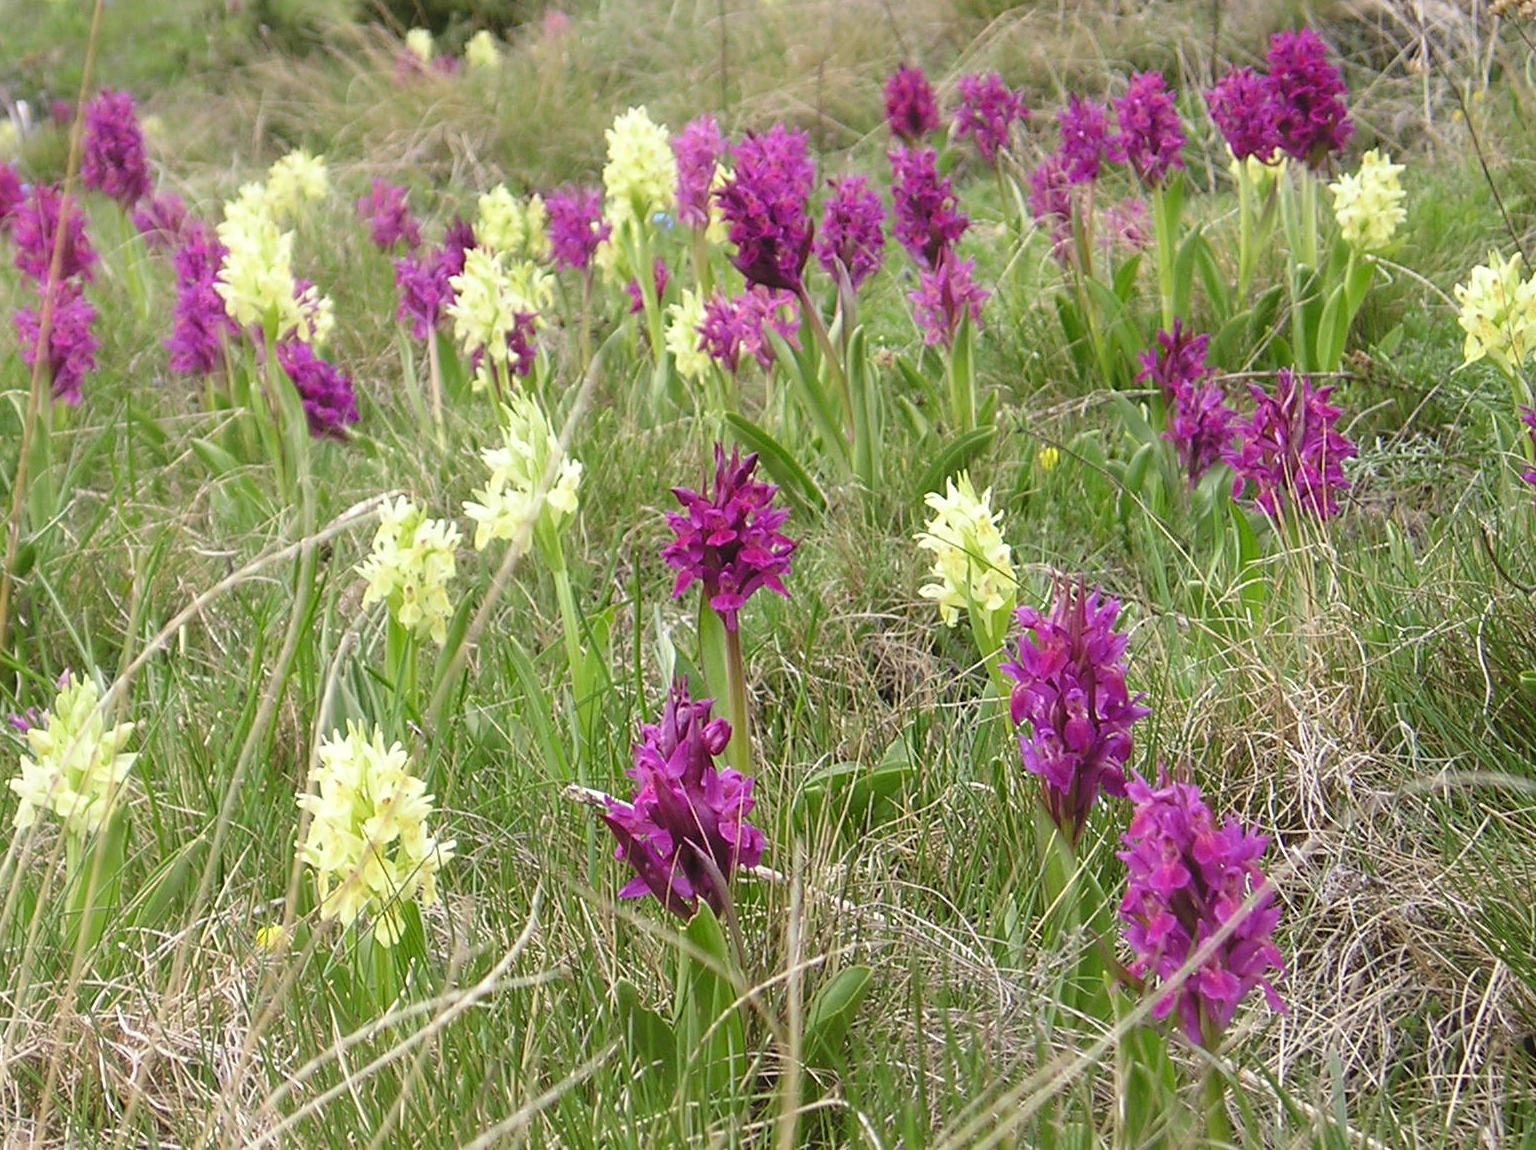
\includegraphics{Species/Dactylorhiza sambucina James D. Ackerman.jpg}

}

\caption{\emph{Dactylorhiza sambucina}. Foto: James D. Ackerman}

\end{figure}%

\begin{center}\rule{0.5\linewidth}{0.5pt}\end{center}

En la siguiente figura se muestra la dinámica de los individuos de
\emph{Listera ovata} muestreados por Tamm desde 1944 a 1971 (Tamm,
1972). En esta figura se puede ver la variabilidad temporal en la
reproducción y supervivencia de las plantas, basado en su presencia o
ausencia, si eran reproductivas o no, reclutamiento e individuos que se
clonan en adición de si las plantas eran latentes. El utilizo un sistema
de presentación de la dinámica de los individuos usando una línea por
individuo y identificando en que etapa estuviese en cada año. El sitio
(plot 48) es bosque mésico con un dosel casi cerrado.

\begin{figure}[H]

{\centering 
\includegraphics[width=0.5\textwidth,height=\textheight]{Figures/Tamm_1972_plot_48.jpeg}

}

\caption{Dinamica del plot 17: Listera ovata, dibujo por Alondra
Martinez Martinez}

\end{figure}%

\begin{center}\rule{0.5\linewidth}{0.5pt}\end{center}

En la publicación de 1972 (Tamm, 1972), Tamm describe la dinámica de
múltiples especies de orquídeas, y algunas especies en múltiples sitios.

\begin{table}
\fontsize{12.0pt}{14.0pt}\selectfont
\begin{tabular*}{\linewidth}{@{\extracolsep{\fill}}lrrr}
\toprule
Especies & N\\'um de la Poblaci\\'on & A\~no del primer muestreo & A\~no del \\'ultimo muestreo \\ 
\midrule\addlinespace[2.5pt]
{\itshape \cellcolor[HTML]{E0FFFF}{Dactylorhiza incarnata}} & 46 & 1944 & 1971 \\ 
{\itshape \cellcolor[HTML]{E0FFFF}{Dactylorhiza sambucina}} & 17 & 1942 & 1971 \\ 
{\itshape \cellcolor[HTML]{E0FFFF}{Dactylorhiza sambucina}} & 18 & 1943 & 1964 \\ 
{\itshape \cellcolor[HTML]{E0FFFF}{Dactylorhiza sambucina}} & 19 & 1943 & 1957 \\ 
{\itshape \cellcolor[HTML]{E0FFFF}{Dactylorhiza sambucina}} & 20 & 1943 & 1957 \\ 
{\itshape \cellcolor[HTML]{E0FFFF}{Dactylorhiza sambucina}} & 21 & 1943 & 1957 \\ 
{\itshape \cellcolor[HTML]{E0FFFF}{Dactylorhiza sambucina}} & 22 & 1943 & 1957 \\ 
{\itshape \cellcolor[HTML]{E0FFFF}{Orchis mascula}} & 24 & 1943 & 1956 \\ 
{\itshape \cellcolor[HTML]{E0FFFF}{Listera ovata}} & 48 & 1944 & 1971 \\ 
\bottomrule
\end{tabular*}
\end{table}

En la publicación de 1972, Tamm describió la dinámica de cuatro especies
de orquídeas. Esta información no están disponible en COMPADRE al
momento. En \emph{Dactylorhiza incarnata} se observa que múltiples
individuos desaparece de un año a otro, que después de 1951 la población
es mayormente vegetativa (sin flores). Usando las figuras, Tamm trató de
ver si había un patrón en la dinámica basado en el cambio de las
comunidades, por ejemplo la presencia de un árbol de pino que se
estableció cerca de la población de \emph{D. sambucina}. La población de
\emph{D. sambucina} disminuyo un poco entre 1942 a 1963, pero fue
balanceado por el reclutamiento de la misma cantidad de individuos en el
mismo periodo. Después de revisar sus datos, Tamm sugirió que lo que
parecen ser individuos nuevos por clonaje pudiese ser realmente nuevos
individuos independiente, solamente muy cerca de un individuo
establecido anteriormente. La dificultad de muestrear con confianza los
individuos en su ambiente es un reto en la interpretación de los datos
de plantas perennes.

\begin{figure}[H]

{\centering 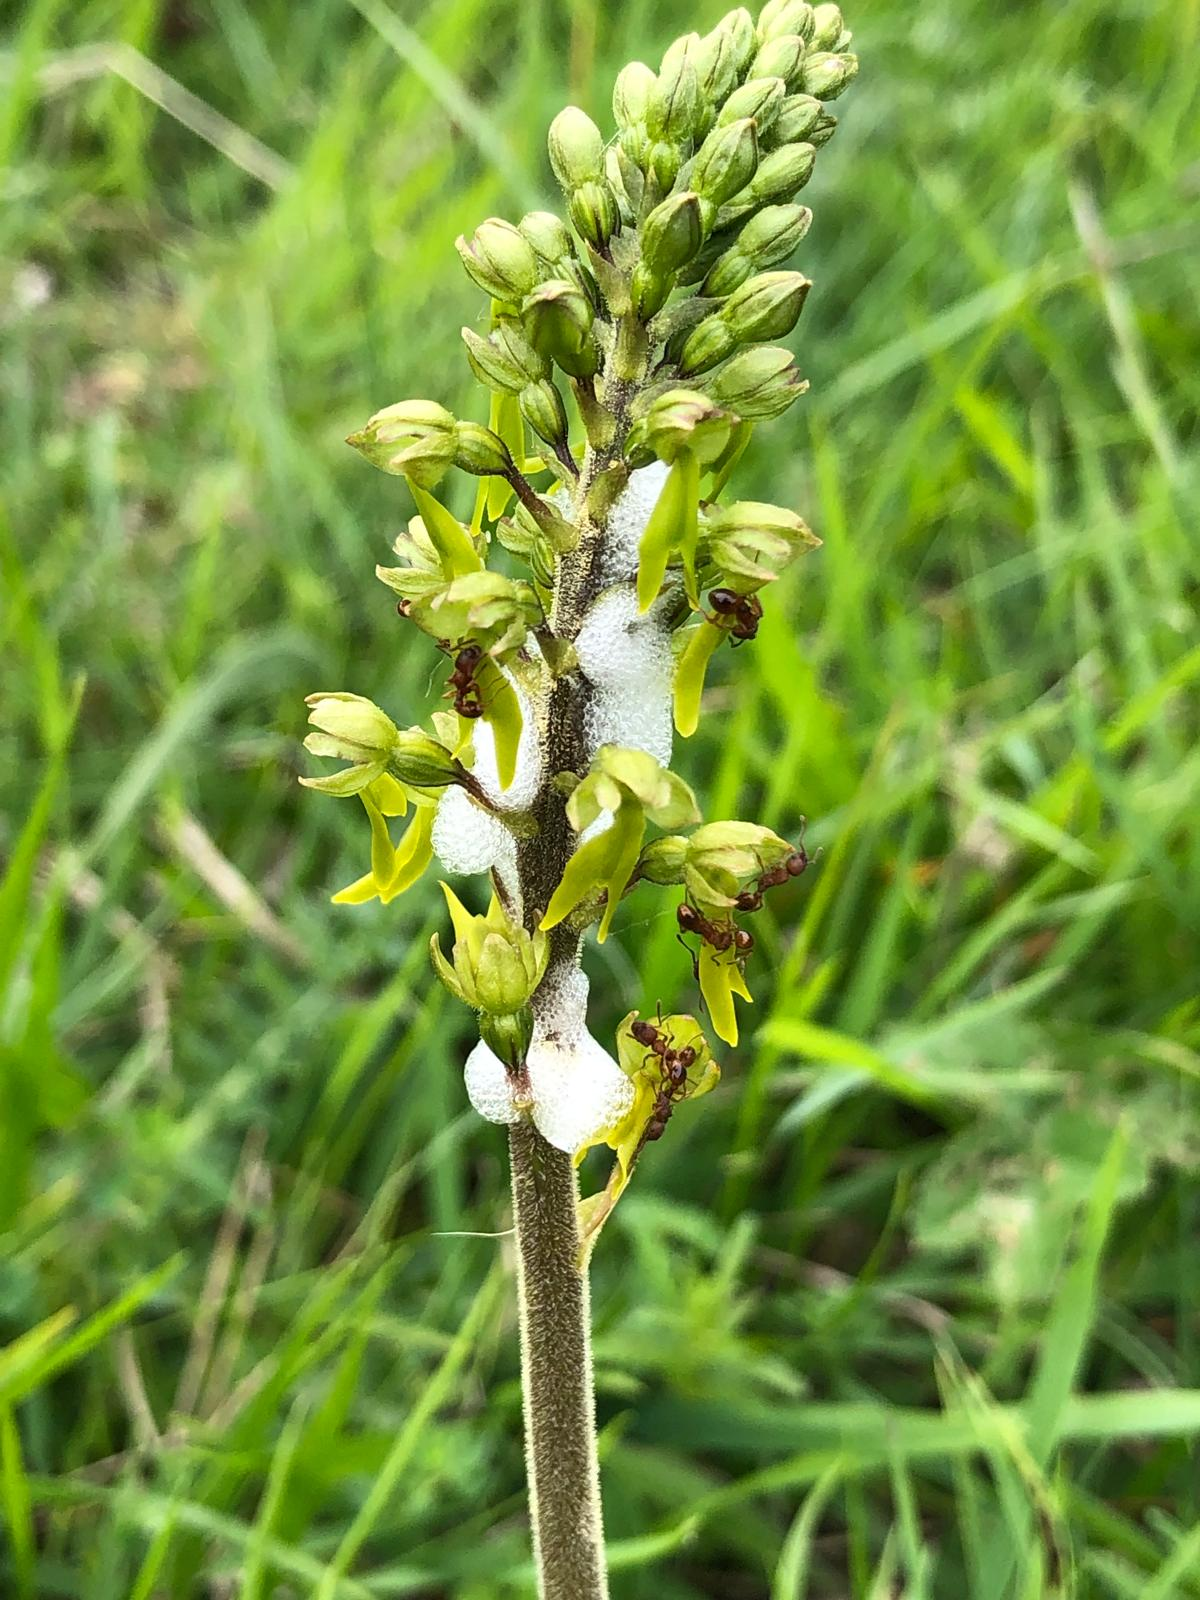
\includegraphics{Species/Dactylorhiza maculata James D. Ackerman.jpg}

}

\caption{\emph{Dactylorhiza maculata con hormigas y spittle bugs}. Foto:
James D. Ackerman}

\end{figure}%

En \emph{Orchis macula}, (ahora \emph{Dactylorhiza maculata}) Tamm
observa claramente que las plantas florecen de forma irregular, y que
parecen tener patrones entre años, que algunos años favorecen la
presencia de inflorescencias y otros años no. En \emph{Listera ovata},
Tamm observó que la población creció, y que hay mucho reclutamiento
entre 1944 y 1971, con un incremento de individuos de más de 200\%
comparando al primer año de muestreo. En adición, él demuestra que hay
individuos que pueden vivir por muchos años. La edad de algunos
individuos de los que el muestreó fue de 30 años para \emph{D.
sambucina}, 28 años para \emph{L. ovata}, 25 años \emph{D. incarnata} y
14 años para \emph{O. mascula}, demostrando que el potencial de largo de
vida para las orquídeas.

Una de las hipótesis de Tamm es que hay senescencia en las orquídeas. En
otra palabra la probabilidad de sobrevivir disminuye con la edad. Él
evaluá el patrón de supervivencia en cuatro especies, \emph{Dactylorhiza
incarnata}, \emph{Dactylorhiza sambucina}, \emph{Listera ovata} y
\emph{Orchis mascula}. Él usó figuras de supervivencia para evaluar la
probabilidad de sobrevivir de un año a otro en una escala logarítmica.
Tamm predijo que si la supervivencia no es ligado a la edad, la
probabilidad de supervivencia debería seguir una línea recta de
mortandad (Tamm, 1972).

\begin{figure}[H]

{\centering 
\includegraphics[width=0.65\textwidth,height=\textheight]{Figures/Tamm_D_sambucina_1945_1970_crop.jpeg}

}

\caption{Supervivencia de Dactylorhiza sambucina}

\end{figure}%

En la figura siguiente se enseña la grafica de supervivencia de
\emph{Dactylorhiza sambucina} muestreado por Tamm desde 1944 a 1971
(re-dibujado por Alondra Martínez Martínez).

\begin{center}\rule{0.5\linewidth}{0.5pt}\end{center}

\section{Re-evaluación de los datos de
Tamm}\label{re-evaluaciuxf3n-de-los-datos-de-tamm}

En la próxima sección se estará re-evaluaron los datos de Tamm con
métodos recientes.

Primero se estará digitalizando los datos, seguido de construcción de
matriz y un análisis sencillo de viabilidad de poblaciones y otras
métricas de dinámica de poblaciones.

\section{Instalación de raretrans
\#2}\label{instalaciuxf3n-de-raretrans-2}

Para instalar \textbf{raretrans} remover el \textbf{\#} antes de correr
el script para tener acceso a los códigos de \textbf{raretrans}. Este
paquete no está disponible en CRAN, pero se puede instalar desde GitHub.

\begin{Shaded}
\begin{Highlighting}[]
\CommentTok{\#devtools::install\_github("atyre2/raretrans", build = TRUE, build\_opts = c("{-}{-}no{-}resave{-}data", "{-}{-}no{-}manual")) \# Instalar el paquete \textquotesingle{}raretrans\textquotesingle{} desde GitHub}
\end{Highlighting}
\end{Shaded}

Subir los datos de Tamm

Se puede tener acceso a los datos de Tamm en el archivo
``Tamm\_1972.xlsx'' en la carpeta ``data'' en Github, de este libro.

Estos datos están limitado a la especie de \emph{Dactylorhiza incarnata}
y se tiene información de los 35 individuos monitoreado en los años 1944
hasta 1971.

\begin{Shaded}
\begin{Highlighting}[]
\NormalTok{Tamm\_1972\_column }\OtherTok{\textless{}{-}} \FunctionTok{read\_excel}\NormalTok{(}\StringTok{"data/Tamm\_1972.xlsx"}\NormalTok{, }
    \AttributeTok{sheet =} \StringTok{"D\_incarnata\_by\_column"}\NormalTok{)}

\NormalTok{Tamm\_1972\_column }\SpecialCharTok{\%\textgreater{}\%} \FunctionTok{head}\NormalTok{()}
\end{Highlighting}
\end{Shaded}

\begin{verbatim}
# A tibble: 6 x 24
  Plant_Num  Year stage next_stage `1948` Fertility `1949` `1950` `1951` `1952`
      <dbl> <dbl> <chr> <chr>      <chr>      <dbl> <chr>  <chr>  <chr>  <chr> 
1         1  1944 F     V          V              0 V      V      V      V     
2         2  1944 F     V          V              0 V      V      V      V     
3         3  1944 F     V          V              0 V      V      V      V     
4         4  1944 F     V          V              0 V      V      V      V     
5         5  1944 V     V          V              0 V      V      F      D     
6         6  1944 V     F          F              0 V      V      V      V     
# i 14 more variables: `1953` <chr>, `1954` <chr>, `1955` <chr>, `1956` <chr>,
#   `1957` <chr>, `1958` <chr>, `59-64` <chr>, `1965` <chr>, `1966` <chr>,
#   `1967` <chr>, `1968` <chr>, `1969` <chr>, `1970` <chr>, `1971` <chr>
\end{verbatim}

El primer paso es encontrar una matriz de valores \emph{prior} para
añadir al modelo de construcción de los parámetros de la matriz. Como no
podemos discutir de estos valores con Tamm, usamos valores de la
literatura. Hay dos especies de \emph{Dactylorhiza} con matrices en
COMPADRE, usando la matriz que más se parece a los datos de los datos de
Tamm, se usó como valores \textbf{prior} los de \emph{Dacylorhiza
lapponica} (Sletvold, Øien \& Moen, 2010). Se modificó la matriz porque
podemos solamente determinar si un individuo falleció después de ser
latente. Entonces la suma de probabilidades de vegetativo y reproductivo
suman a 1.0 y los latentes no suma a 1.0 (la diferencia es los
fallecidos).

\begin{Shaded}
\begin{Highlighting}[]
\NormalTok{Dacty\_apriori}\OtherTok{=}\FunctionTok{matrix}\NormalTok{(}\FunctionTok{c}\NormalTok{(}\FloatTok{0.637}\NormalTok{, }\FloatTok{0.571}\NormalTok{, }\FloatTok{0.740}\NormalTok{,}
                       \FloatTok{0.273}\NormalTok{, }\FloatTok{0.271}\NormalTok{, }\FloatTok{0.049}\NormalTok{,}
                       \FloatTok{0.090}\NormalTok{, }\FloatTok{0.158}\NormalTok{, }\FloatTok{0.059}\NormalTok{,}
                       \DecValTok{0}\NormalTok{,     }\DecValTok{0}\NormalTok{,     }\FloatTok{0.152}\NormalTok{),  }
              \AttributeTok{nrow =} \DecValTok{4}\NormalTok{, }\AttributeTok{ncol =} \DecValTok{3}\NormalTok{, }
              \AttributeTok{byrow=}\ConstantTok{TRUE}\NormalTok{) }\CommentTok{\# la última fila es la proporción de individuos en esta etapa que fallece. }

\NormalTok{Dacty\_apriori}
\end{Highlighting}
\end{Shaded}

\begin{verbatim}
      [,1]  [,2]  [,3]
[1,] 0.637 0.571 0.740
[2,] 0.273 0.271 0.049
[3,] 0.090 0.158 0.059
[4,] 0.000 0.000 0.152
\end{verbatim}

\section{Construcción de la matriz de
transición}\label{construcciuxf3n-de-la-matriz-de-transiciuxf3n}

\begin{itemize}
\item
  Las etapas en el modelo son Vegetativo (sin flores), Floreciendo (con
  flores), y Latente (no avistamiento en un año particular) en adición
  que los individuos fallecidos.
\item
  La matriz de transiciones es una matriz de 3 x 3, donde las filas son
  las etapas futuras (tiempo t+1) y las columnas son las etapas actuales
  (tiempo t).
\item
  Debido a la poca cantidad de datos se estará haciendo una matriz de
  todos los datos juntos, no se estará considerando la variación inter
  anual. Pero los datos están disponibles por años también en la hoja de
  Excel y si desean pueden evaluar la variación inter-anual.
\item
  Se usarán las columnas ``stage'' etapa en el tiempo \(t\) y
  ``next\_stage'' etapa en el tiempo \(t_{+1}\).
\item
  Supuestos del modelo:

  \begin{itemize}
  \tightlist
  \item
    Que los individuos no pueden ser latentes más de dos años
    consecutivos. Todo individuo que no es visto después de dos años es
    considerado fallecido. Ese supuesto proviene de haber evaluado la
    figura de Tamm y ver que no hay individuos que sean vistos después
    de dos años consecutivos de ser latentes.
  \item
    Naturalmente el supuesto más significativo aquí es que el tamaño de
    muestra es suficiente para capturar los eventos raros (por ejemplos
    los individuos que sean latentes más de dos años consecutivos).
  \item
    Un individuo fallecido no puede regresar en un estado en el futuro
    (una condición lógica).
  \end{itemize}
\end{itemize}

\begin{Shaded}
\begin{Highlighting}[]
\NormalTok{Tmat\_D }\OtherTok{\textless{}{-}}\NormalTok{ Tamm\_1972\_column }\SpecialCharTok{\%\textgreater{}\%}
\NormalTok{  dplyr}\SpecialCharTok{::}\FunctionTok{select}\NormalTok{(Year, stage, next\_stage, Fertility) }\SpecialCharTok{\%\textgreater{}\%}
  \FunctionTok{mutate}\NormalTok{(}
    \AttributeTok{stage =} \FunctionTok{factor}\NormalTok{(stage, }\AttributeTok{levels =} \FunctionTok{c}\NormalTok{(}\StringTok{"V"}\NormalTok{, }\StringTok{"F"}\NormalTok{, }\StringTok{"D"}\NormalTok{, }\StringTok{"m"}\NormalTok{)),}
    \AttributeTok{fate =} \FunctionTok{factor}\NormalTok{(next\_stage, }\AttributeTok{levels =} \FunctionTok{c}\NormalTok{(}\StringTok{"V"}\NormalTok{, }\StringTok{"F"}\NormalTok{, }\StringTok{"D"}\NormalTok{, }\StringTok{"m"}\NormalTok{))}
\NormalTok{  ) }\SpecialCharTok{\%\textgreater{}\%}
  \FunctionTok{drop\_na}\NormalTok{(stage, fate) }\SpecialCharTok{\%\textgreater{}\%}
  \FunctionTok{as.data.frame}\NormalTok{() }\SpecialCharTok{\%\textgreater{}\%}
  \FunctionTok{xtabs}\NormalTok{(}\SpecialCharTok{\textasciitilde{}}\NormalTok{ fate }\SpecialCharTok{+}\NormalTok{ stage, }\AttributeTok{data =}\NormalTok{ .) }\SpecialCharTok{\%\textgreater{}\%}
  \FunctionTok{as.matrix}\NormalTok{()}

\NormalTok{Tmat\_D }\CommentTok{\# se contabiliza la cantidad de individuos que pasan de una etapa a otra para todos los años (no se considerá la variación inter anual).}
\end{Highlighting}
\end{Shaded}

\begin{verbatim}
    stage
fate   V   F   D   m
   V 128   6   6   0
   F   3   0   0   0
   D  40   1   1   0
   m   0   0  30   0
\end{verbatim}

\begin{Shaded}
\begin{Highlighting}[]
\NormalTok{Tmat2 }\OtherTok{\textless{}{-}}\NormalTok{ Tmat\_D[, }\SpecialCharTok{{-}}\DecValTok{4}\NormalTok{] }\CommentTok{\# remover la columna para transiciones de la muerte (es imposible pasar de fallecido a otra etapas)}
\NormalTok{Tmat2}
\end{Highlighting}
\end{Shaded}

\begin{verbatim}
    stage
fate   V   F   D
   V 128   6   6
   F   3   0   0
   D  40   1   1
   m   0   0  30
\end{verbatim}

\begin{Shaded}
\begin{Highlighting}[]
\NormalTok{N2\_D }\OtherTok{\textless{}{-}} \FunctionTok{colSums}\NormalTok{(Tmat2) }\CommentTok{\# obtener el número total de una etapa.}
\NormalTok{N2\_D}
\end{Highlighting}
\end{Shaded}

\begin{verbatim}
  V   F   D 
171   7  37 
\end{verbatim}

\begin{Shaded}
\begin{Highlighting}[]
\NormalTok{Tmat }\OtherTok{\textless{}{-}} \FunctionTok{sweep}\NormalTok{(Tmat2[}\SpecialCharTok{{-}}\DecValTok{4}\NormalTok{, ], }\DecValTok{2}\NormalTok{, N2\_D, }\StringTok{"/"}\NormalTok{) }\CommentTok{\# normalizar las transiciones, nota que el "2" es para decir que haga los cálculos por columna (en este caso división por la cantidad total de individuos en la etapa)}
\NormalTok{Tmat }\CommentTok{\# la matriz de transición final normalizada con los datos del campo}
\end{Highlighting}
\end{Shaded}

\begin{verbatim}
    stage
fate          V          F          D
   V 0.74853801 0.85714286 0.16216216
   F 0.01754386 0.00000000 0.00000000
   D 0.23391813 0.14285714 0.02702703
\end{verbatim}

\section{Apreciación de la matriz}\label{apreciaciuxf3n-de-la-matriz}

\begin{itemize}
\tightlist
\item
  La mayoría de los individuos en la población de \emph{Dactylorhiza
  incarnata} son vegetativos (sin flores) y están en estado vegetativo
  (sin flores) y siguen en dicho estado el próximo periodo.
\item
  La mayoría de los individuos que florecen en un año particular no
  florecen en el año siguiente.
\item
  Solamente 16\% de los individuos latentes en año particular son
  vegetativos el próximo año y ninguno de los individuos latentes un año
  particular florecen el año siguiente.
\end{itemize}

\begin{center}\rule{0.5\linewidth}{0.5pt}\end{center}

\section{Construcción de la matriz de
fertilidad}\label{construcciuxf3n-de-la-matriz-de-fertilidad}

Para tomar en cuenta la fecundidad, se necesita una matriz de
fertilidad. En este caso los datos son muy limitados, tenemos solamente
la cantidad de individuos que florecieron en 1944. Para simplificar, se
asume que la cantidad de individuos que florecieron en 1944 (n=5), 1948
(n=1), 1949 (n=2) y 1951 (n=1) es la cantidad de semillas que producen.
Solamente el individuo \#5 se reprodujo dos veces. Asumimos que todos
los nuevos individuos en la población provienen de estos individuos
floreciendo y que ningún reclutamiento proviene de fuentes externas,
entonces la matriz de fertilidad es la siguiente. De 9 individuos
florecidos tenemos 15 individuos nuevos entre 1949 a 1967. Nota aquí que
no es la cantidad de semillas producidas, por que no tenemos la
información sobre la cantidad de semillas que germinan y se establecen.
Lo que tenemos es la cantidad de individuos que florecen y por
consecuencia producen nuevos individuos vegetativos. El cálculo es 15
individuos nuevos por 9 individuos florecidos = 1.667 individuos nuevos
por individuo florecido. El otro supuesto es que las semillas pueden ser
latentes por múltiples años; o se puede que germinen pero no producen
individuos vegetativos o con flores inmediatamente, entonces un periodo
de latencia después de germinar (una etapa no observada: esa etapa no
está en el modelo).

\begin{itemize}
\tightlist
\item
  La latencia de las semillas de orquídeas es un supuesto que no se
  puede evaluar con los datos de Tamm, pero es un supuesto razonable si
  uno toma en cuenta los trabajos de Whigham et al. (Whigham et al.,
  2006).
\end{itemize}

\section{Crear la matriz de
fecundidad}\label{crear-la-matriz-de-fecundidad}

\begin{Shaded}
\begin{Highlighting}[]
\NormalTok{Fmat }\OtherTok{\textless{}{-}} \FunctionTok{matrix}\NormalTok{(}\DecValTok{0}\NormalTok{, }\AttributeTok{nrow =} \DecValTok{3}\NormalTok{, }\AttributeTok{ncol =} \DecValTok{3}\NormalTok{) }\CommentTok{\# crear una matriz de ceros.}
\NormalTok{Fmat[}\DecValTok{1}\NormalTok{, }\DecValTok{2}\NormalTok{] }\OtherTok{\textless{}{-}} \DecValTok{15} \SpecialCharTok{/} \DecValTok{9} \CommentTok{\# contar 9 adultos reproductivos en el tiempo t y 15 nuevos individuos en el tiempo t+i en la población. Añadir el valor en la posición correcta de la matriz de fertilidad (nnota es la primera fila, segunda columna).}

\NormalTok{TF2 }\OtherTok{\textless{}{-}} \FunctionTok{list}\NormalTok{(}\AttributeTok{Tmat =}\NormalTok{ Tmat, }\AttributeTok{Fmat =}\NormalTok{ Fmat) }\CommentTok{\# crear una lista con las matrices de transiciones y de fertilidad.}
\NormalTok{TF2}
\end{Highlighting}
\end{Shaded}

\begin{verbatim}
$Tmat
    stage
fate          V          F          D
   V 0.74853801 0.85714286 0.16216216
   F 0.01754386 0.00000000 0.00000000
   D 0.23391813 0.14285714 0.02702703

$Fmat
     [,1]     [,2] [,3]
[1,]    0 1.666667    0
[2,]    0 0.000000    0
[3,]    0 0.000000    0
\end{verbatim}

\begin{center}\rule{0.5\linewidth}{0.5pt}\end{center}

¿Como se ve el ciclo de vida de esa especie en estos años?

\begin{itemize}
\tightlist
\item
  rojo: individuos que se quedan en la misma etapa
\item
  verde: individuos que pasan de una etapa a otra (excluyendo latente)
\item
  azul: individuos que pasan de una etapa a latente
\item
  amarillo: individuos que producen nuevos individuos en la población
\end{itemize}

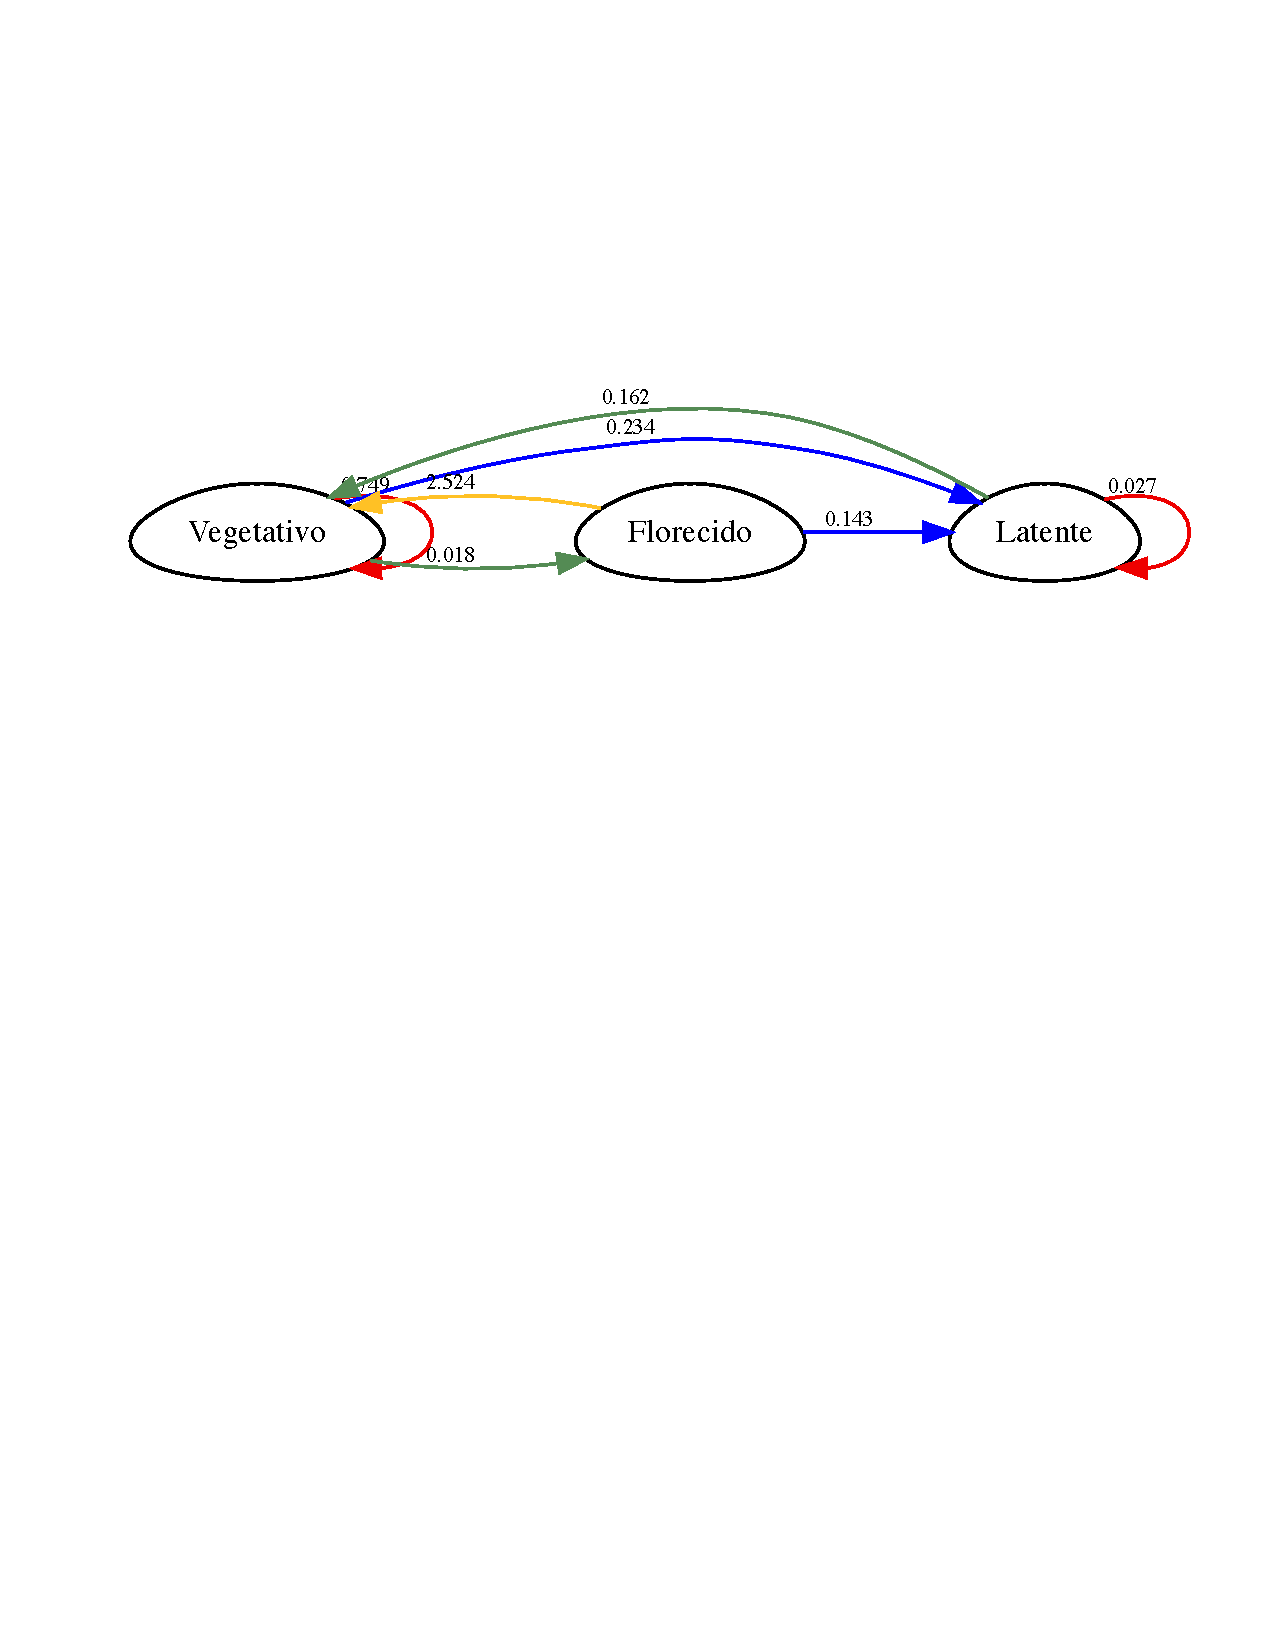
\includegraphics{118-Carl_Olaf_Tamm_files/figure-pdf/OCTamm_11-1.pdf}

\begin{center}\rule{0.5\linewidth}{0.5pt}\end{center}

\section{Análisis de viabilidad de
poblaciones}\label{anuxe1lisis-de-viabilidad-de-poblaciones}

Ahora usamos la información de las matrices de transiciones,
fertilidades y sus valores de prior para calcular los parámetros de la
especie

Antes de seguir, comparamos la matriz original con los valores de la
matriz posterior. Para calcular la matriz de transición y de fecundidad
posterior se usa la función ``priorweight'' para reducir o aumentar la
confianza que uno tiene sobre los valores prior. Nota que como estos
valores provienen de otra especies es buena idea reducir la confianza
que uno tiene sobre estos valores de ``priors'' en los análisis usando
un \textbf{priorweight} pequeño.

El valor de 0.01, es que se usa 1\% de los valores prior y 99\% de los
valores del campo. Por consecuencia dominará los valores del campo. Nota
que en la matriz posterior se observa valores en parámetros que
originalmente eran cero (ejemplo: plantas con flores que se queden con
flores, valores que no se observaron del campo). Nota ahora tenemos un
valor de 2\% de individuos que florecen en un año particular que se
quedan con flores en el año siguiente. Eso no fue un valor observado en
los datos de campo, pero es un valor que se puede calcular con los datos
que tenemos, y es probable que sea realista ya que ocurre en otras
especies de orquídeas del mismo género. Nota también que hay una pequeña
probabilidad que una planta latente sea fértil en el año siguiente
(0.004).

\begin{Shaded}
\begin{Highlighting}[]
\NormalTok{TF2}\SpecialCharTok{$}\NormalTok{Tmat}
\end{Highlighting}
\end{Shaded}

\begin{verbatim}
    stage
fate          V          F          D
   V 0.74853801 0.85714286 0.16216216
   F 0.01754386 0.00000000 0.00000000
   D 0.23391813 0.14285714 0.02702703
\end{verbatim}

\begin{Shaded}
\begin{Highlighting}[]
\NormalTok{TF3}\OtherTok{=}\FunctionTok{fill\_transitions}\NormalTok{(TF2, N2\_D, }\AttributeTok{P =}\NormalTok{ Dacty\_apriori, }\AttributeTok{priorweight =} \FloatTok{0.1}\NormalTok{)}

\NormalTok{TF3 }\CommentTok{\# la matriz de transiciones posterior}
\end{Highlighting}
\end{Shaded}

\begin{verbatim}
           [,1]       [,2]        [,3]
[1,] 0.73839819 0.83112987 0.214692875
[2,] 0.04076715 0.02463636 0.004454545
[3,] 0.22083466 0.14423377 0.029933661
\end{verbatim}

El estimado de \(\lambda\)

Como es esperado, la población de \emph{Dactylorhiza incarnata}
disminuye en el tiempo y el indice de crecimiento es menor que 1.0. El
valor de crecimiento intrínsico es de 0.84, que siguiere una disminución
de la población de aproximadamente 16\% por año. Era de esperar que el
crecimiento poblacional sea menor que 1.0, ya que la mayoría de los
individuos en la población son vegetativos y que la mayoría de los
individuos que florecen en un año particular no florecen en el año
siguiente, hay poco reclutamiento y el nivel de mortandad es alta.

\begin{Shaded}
\begin{Highlighting}[]
\NormalTok{popbio}\SpecialCharTok{::}\FunctionTok{lambda}\NormalTok{(TF3)}
\end{Highlighting}
\end{Shaded}

\begin{verbatim}
[1] 0.8415307
\end{verbatim}

\section{Simulando el crecimiento
poblacional}\label{simulando-el-crecimiento-poblacional}

Uno de los retos en los análisis de viabilidad de población es la
construcción de intervalos de confianza. El valor anterior de lambda es
un valor puntual, pero no nos dice nada sobre la variabilidad de los
datos. Para calcular el intervalo de confianza se puede hacer una
simulación de Monte Carlo. En este caso se simula el crecimiento
poblacional de \emph{Dactylorhiza incarnata} muestreado por Tamm desde
1944 a 1971. Pero esta vez se usará información para hacer un modelo
completamente bayesiano. La ventaja es que los valores de credibilidad
de los parámetros son más informativos y se basando en la incertidumbre
las transiciones.

Para estimar los intervalos de credibilidad se simula la matriz, tomando
en consideración el tamaño de muestra (N2\_d), las matriz de los valores
del campo (TF2), la matriz de los valores prior (Dacty\_apriori), el
peso de los valores prior (priorweight), los prior de fertilidad y la
cantidad de simulaciones (samples = 5000) que queremos generar (Para
determinar la cantidad de simulaciones se puede correr el análisis
múltiples veces y evaluar si aumentando la simulaciones impacta los
intervalos de credibilidad) . Con esta simulación podemos calcular el
intervalo decredibilidad del crecimiento poblacional de
\emph{Dactylorhiza incarnata} muestreado por Tamm desde 1944 a 1971.

Las matrices alpha2 y beta2, representan los parámetros de la
distribución gamma con media alpha/beta. En este caso se usa valores muy
pequeños para los valores alpha y beta, para que la distribución gamma
no sea informativa (non-informative priors) y que los valores de lambda
sean muy dispersos. En otras palabras no ponemos mucho peso en los
valores prior de la fertilidad, y dejamos que los valores del campo
dominen los análisis.

\begin{Shaded}
\begin{Highlighting}[]
\NormalTok{alpha2 }\OtherTok{\textless{}{-}} \FunctionTok{matrix}\NormalTok{(}\FunctionTok{c}\NormalTok{(}\ConstantTok{NA\_real\_}\NormalTok{, }\FloatTok{1e{-}5}\NormalTok{,     }\ConstantTok{NA\_real\_}\NormalTok{,}
                   \ConstantTok{NA\_real\_}\NormalTok{, }\ConstantTok{NA\_real\_}\NormalTok{, }\ConstantTok{NA\_real\_}\NormalTok{,}
                   \ConstantTok{NA\_real\_}\NormalTok{, }\ConstantTok{NA\_real\_}\NormalTok{, }\ConstantTok{NA\_real\_}\NormalTok{), }
          \AttributeTok{nrow=}\DecValTok{3}\NormalTok{, }\AttributeTok{ncol =} \DecValTok{3}\NormalTok{, }
          \AttributeTok{byrow =} \ConstantTok{TRUE}\NormalTok{) }\CommentTok{\# la matriz de los valores alpha}
\NormalTok{beta2 }\OtherTok{\textless{}{-}} \FunctionTok{matrix}\NormalTok{(}\FunctionTok{c}\NormalTok{( }\ConstantTok{NA\_real\_}\NormalTok{, }\FloatTok{1e{-}5}\NormalTok{,     }\ConstantTok{NA\_real\_}\NormalTok{,}
                   \ConstantTok{NA\_real\_}\NormalTok{, }\ConstantTok{NA\_real\_}\NormalTok{, }\ConstantTok{NA\_real\_}\NormalTok{,}
                   \ConstantTok{NA\_real\_}\NormalTok{, }\ConstantTok{NA\_real\_}\NormalTok{, }\ConstantTok{NA\_real\_}\NormalTok{), }
          \AttributeTok{nrow=}\DecValTok{3}\NormalTok{, }\AttributeTok{ncol =} \DecValTok{3}\NormalTok{, }
          \AttributeTok{byrow =} \ConstantTok{TRUE}\NormalTok{) }\CommentTok{\# la matriz de los valores beta}
\end{Highlighting}
\end{Shaded}

Ahora unimos todos los valores, para simular el crecimiento poblacional
de \emph{Dactylorhiza incarnata} con la función
\textbf{sim\_transitions} muestreado por Tamm desde 1944 a 1971.

\begin{itemize}
\tightlist
\item
  \textbf{TF2} es la matriz de transiciones y de fertilidades
\item
  \textbf{N2\_D} es el vector de la cantidad de individuos en cada etapa
\item
  \textbf{Dacty\_apriori} es la matriz de los valores prior
\item
  \textbf{alpha2} y \textbf{beta2} son los valores de los parámetros de
  la distribución gamma para la fertilidad
\item
  \textbf{priorweight} es el peso de los valores prior
\item
  \textbf{samples} es la cantidad de simulaciones que queremos generar.
\end{itemize}

\begin{Shaded}
\begin{Highlighting}[]
\NormalTok{Dacty\_0}\FloatTok{.1} \OtherTok{\textless{}{-}} \FunctionTok{sim\_transitions}\NormalTok{(}
\NormalTok{  TF2,}
\NormalTok{  N2\_D,}
  \AttributeTok{P =}\NormalTok{ Dacty\_apriori,}
  \AttributeTok{alpha =}\NormalTok{ alpha2,}
  \AttributeTok{beta =}\NormalTok{ beta2,}
  \AttributeTok{priorweight =} \FloatTok{0.1}\NormalTok{,}
  \AttributeTok{samples =} \DecValTok{5000}
\NormalTok{) }\CommentTok{\# generar 5000 matrices basado en las previas de transiciones y de fertilidades, el tamaño de muestra, en adición de los datos}
\end{Highlighting}
\end{Shaded}

Se convierte el objeto ``Dacty\_0.1'' en un tibble para poder visualizar
la distribución de los lambda que proviene de la simulación.

\begin{Shaded}
\begin{Highlighting}[]
\NormalTok{Dacty\_0}\FloatTok{.1}\NormalTok{b }\OtherTok{\textless{}{-}} \FunctionTok{tibble}\NormalTok{(}\AttributeTok{lposterior =} \FunctionTok{map\_dbl}\NormalTok{(Dacty\_0}\FloatTok{.1}\NormalTok{, lambda))}
\end{Highlighting}
\end{Shaded}

\section{Visualización de las distribuciones de los
lambda.}\label{visualizaciuxf3n-de-las-distribuciones-de-los-lambda.}

Se nota claramente que la población de \emph{Dactylorhiza incarnata}
muestreado por Tamm desde 1944 a 1971 tiene un crecimiento poblacional
menor que 1.0. Nota que esta simulación considera variación demográfica
en los datos.

\begin{Shaded}
\begin{Highlighting}[]
\FunctionTok{ggplot}\NormalTok{(}\AttributeTok{data =}\NormalTok{ Dacty\_0}\FloatTok{.1}\NormalTok{b, }\AttributeTok{mapping =} \FunctionTok{aes}\NormalTok{(}\AttributeTok{x =}\NormalTok{ lposterior)) }\SpecialCharTok{+}
  \FunctionTok{geom\_histogram}\NormalTok{(}\AttributeTok{binwidth =} \FloatTok{0.01}\NormalTok{, }\AttributeTok{colour =} \StringTok{"white"}\NormalTok{) }\SpecialCharTok{+}
  \FunctionTok{rlt\_style\_colour}\NormalTok{() }\SpecialCharTok{+}
  \FunctionTok{geom\_vline}\NormalTok{(}\AttributeTok{xintercept =} \DecValTok{1}\NormalTok{, }\AttributeTok{color =} \StringTok{"\#009392"}\NormalTok{, }\AttributeTok{size =} \FloatTok{1.5}\NormalTok{)}
\end{Highlighting}
\end{Shaded}

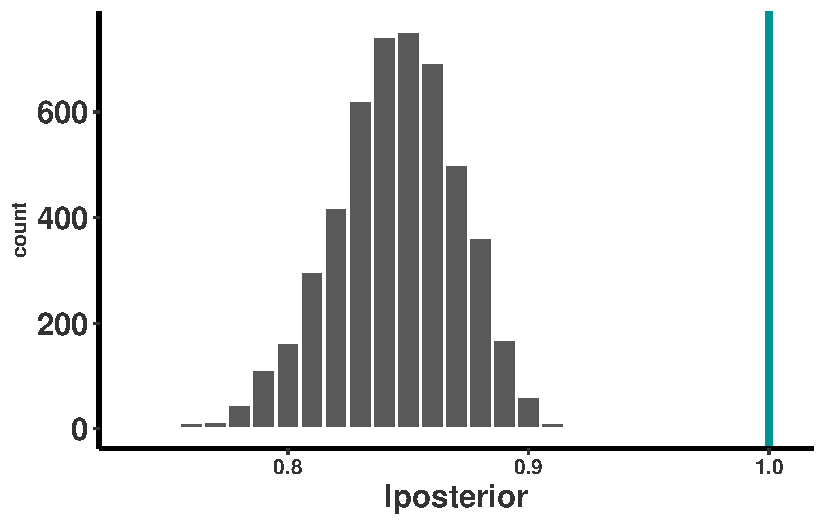
\includegraphics{118-Carl_Olaf_Tamm_files/figure-pdf/OCTamm_17-1.pdf}

Para concluir, la población de \emph{Dactylorhiza incarnata} muestreado
por Tamm desde 1944 a 1971 tiene un crecimiento poblacional menor que
1.0 (lambda promedio de 0.84), con un intervalo de confianza de 0.79 a
0.89. Esto indica que la población esta reduciendo en el tiempo por
aproximadamente 16\%, pero que realmente la reducción pudiese ser entre
21\% a 11\%. El índice de \emph{pincrease} es el valor de \emph{p} para
evaluar si la población esta creciendo o decreciendo. En este caso el
valor es \textless0.001, lo que indica que la población está
decreciendo.

\begin{Shaded}
\begin{Highlighting}[]
\NormalTok{Dacty\_0}\FloatTok{.1}\NormalTok{bdf }\OtherTok{=} \FunctionTok{as.data.frame}\NormalTok{(Dacty\_0}\FloatTok{.1}\NormalTok{b)}
\NormalTok{Dacty\_0}\FloatTok{.1}\NormalTok{\_summary }\OtherTok{\textless{}{-}}\NormalTok{ dplyr}\SpecialCharTok{::}\FunctionTok{summarize}\NormalTok{(}
\NormalTok{  Dacty\_0}\FloatTok{.1}\NormalTok{bdf,}
  \AttributeTok{medianL =} \FunctionTok{median}\NormalTok{(lposterior),}
  \AttributeTok{meanL =} \FunctionTok{mean}\NormalTok{(lposterior),}
  \AttributeTok{lcl =} \FunctionTok{quantile}\NormalTok{(lposterior, }\AttributeTok{probs =} \FloatTok{0.025}\NormalTok{),}
  \AttributeTok{ucl =} \FunctionTok{quantile}\NormalTok{(lposterior, }\AttributeTok{probs =} \FloatTok{0.975}\NormalTok{),}
  \AttributeTok{pincrease =} \FunctionTok{sum}\NormalTok{(lposterior }\SpecialCharTok{\textgreater{}} \FloatTok{1.}\NormalTok{) }\SpecialCharTok{/} \FunctionTok{n}\NormalTok{()}
\NormalTok{)}
\end{Highlighting}
\end{Shaded}

\begin{Shaded}
\begin{Highlighting}[]
\FunctionTok{gt}\NormalTok{(}\FunctionTok{signif}\NormalTok{(Dacty\_0}\FloatTok{.1}\NormalTok{\_summary, }\AttributeTok{digits =} \DecValTok{3}\NormalTok{))}
\end{Highlighting}
\end{Shaded}

\begin{table}
\fontsize{12.0pt}{14.0pt}\selectfont
\begin{tabular*}{\linewidth}{@{\extracolsep{\fill}}rrrrr}
\toprule
medianL & meanL & lcl & ucl & pincrease \\ 
\midrule\addlinespace[2.5pt]
0.846 & 0.845 & 0.79 & 0.891 & 0 \\ 
\bottomrule
\end{tabular*}
\end{table}

Revisión RLT: Oct 7, 2024

Revisión RLT: Oct 8, 2024

Revisión RLT: Oct 30, 2024

Revisión RLT: el 26 de Noviembre, 2024

Revisión RLT: el 18 de enero, 2025

Revisión Joel Tupac: el 5 de junio, 2025

\phantomsection\label{refs}
\begin{CSLReferences}{1}{0}
\bibitem[\citeproctext]{ref-sletvold2010long}
Sletvold N, Øien D-I, Moen A. 2010. Long-term influence of mowing on
population dynamics in the rare orchid \emph{{D}actylorhiza
{l}apponica}: The importance of recruitment and seed production.
\emph{Biological Conservation} 143:747--755.

\bibitem[\citeproctext]{ref-tamm1948observations}
Tamm CO. 1948. Observations on reproductive and survival of some
perrenial herbs. \emph{Botanish Notiser}:305--321.

\bibitem[\citeproctext]{ref-tamm1956further}
Tamm CO. 1956. Further observations on the survival and flowering of
some perennial herbs, i. \emph{Oikos} 7:273--292.

\bibitem[\citeproctext]{ref-tamm1972survival}
Tamm CO. 1972. Survival and flowering of some perennial herbs. II. The
behaviour of some orchids on permanent plots. \emph{Oikos}:23--28.

\bibitem[\citeproctext]{ref-whigham2006seed}
Whigham DF, O'Neill JP, Rasmussen HN, Caldwell BA, McCormick MK. 2006.
Seed longevity in terrestrial orchids--potential for persistent in situ
seed banks. \emph{Biological Conservation} 129:24--30.

\end{CSLReferences}


\backmatter


\end{document}
